% Provisional development evidence; no independent generalization claim.
\begin{figure*}[t]
\centering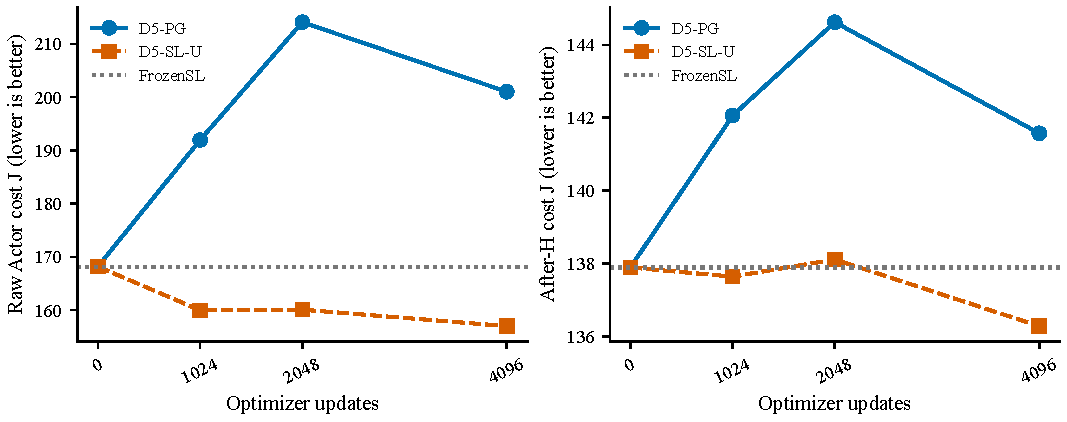
\includegraphics[width=.95\textwidth]{rc3_d5_revision_20261112/figures/fixed_endpoint_quality.pdf}
\caption{Fixed-endpoint complete-task cost on 66 exposed development requests from 11 parent layouts and one prespecified seed. Six requests are averaged within each parent, then parents receive equal weight. Raw and after-H cost are shown separately; $J=L+0.75K$ is measured in metre-equivalent cost units, where $L$ is navigation length in metres and $K$ counts stops. Smaller is better. The shared zero-update point is the exact SL256 baseline. Only update4096 determines P1.}
\label{fig:d5-fixed-endpoints}
\end{figure*}
\begin{figure*}[t]
\centering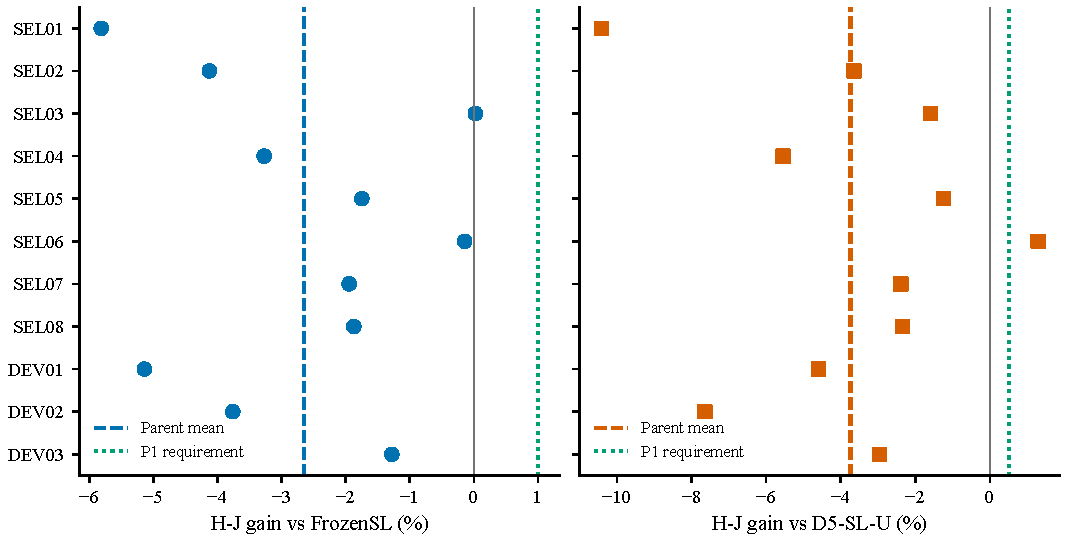
\includegraphics[width=.95\textwidth]{rc3_d5_revision_20261112/figures/parent_paired_HJ.pdf}
\caption{Parent-paired after-H J gains of D5-PG at update4096 over FrozenSL and update/exposure-matched SL-U. Each parent averages six requests; positive values indicate improvement. Dashed lines mark parent means and dotted lines mark the original P1 thresholds. SEL and DEV are both exposed development data.}
\label{fig:d5-parent-gains}
\end{figure*}
\begin{figure*}[t]
\centering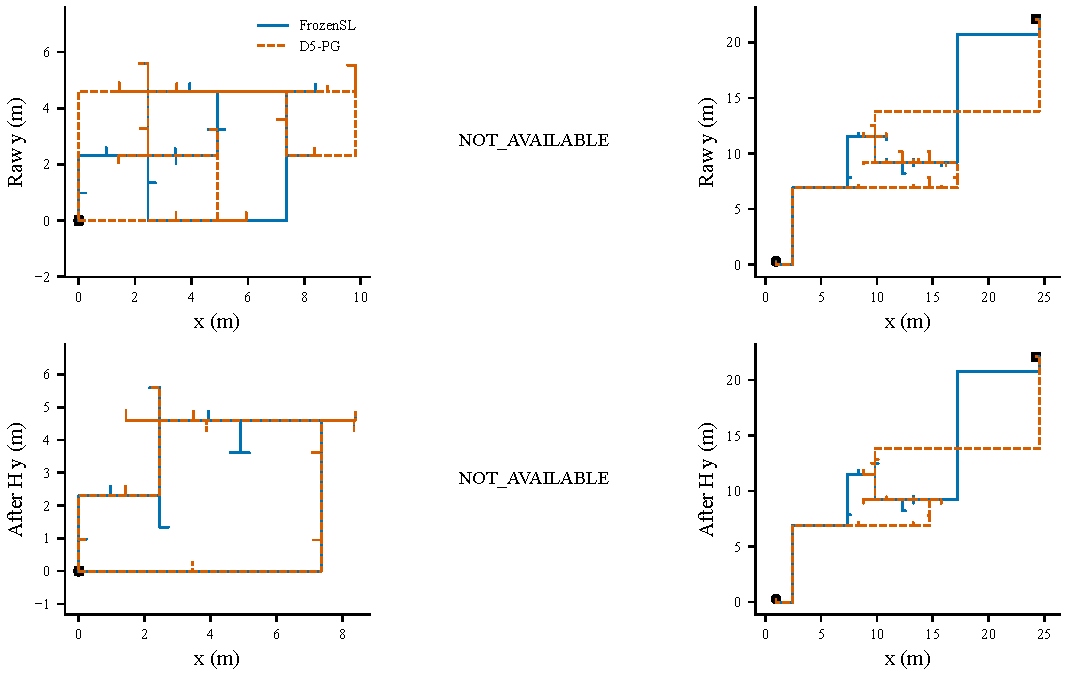
\includegraphics[width=.95\textwidth]{rc3_d5_revision_20261112/figures/saved_route_examples.pdf}
\caption{Saved navigation polylines for update4096 D5-PG and FrozenSL, with raw routes above and after-H routes below. Columns select the lexicographically first case ID with improved, equal, or degraded after-H $J$, using absolute equality tolerance $10^{-8}$ metre-equivalent units. The 66 cases comprise 22 improved, zero tied, and 44 degraded cases; the selected cases are development\_000, unavailable, and development\_001. Missing categories remain unavailable. The complete 66-case statistics determine the result; these are not new planning calls or certified arm trajectories.}
\label{fig:d5-saved-routes}
\end{figure*}
